\documentclass[runningheads]{llncs}
\usepackage{graphicx,amssymb,pepa,pgfplots,pgfplotstable,amsmath,placeins}
\usetikzlibrary{patterns}

% ---- Highlighting placeholder text
\usepackage{xcolor}
\usepackage{framed}
\colorlet{shadecolor}{red!20}


\begin{document}
\title{Performance modelling and simulation of skewed demand in complex systems}

\author{Stephen Shephard}

\institute{School of Computing Science, Newcastle University, Newcastle upon Tyne, NE1 7RU\\
	\email{s.shephard2@newcastle.ac.uk}}

\maketitle

%
% ---- Abstract and keywords
%
\begin{shaded}
\begin{abstract}
On-line Transaction Processing (OLTP) applications must frequently deal with the issue of skewed demand for some resources.  This demand may overwhelm the whole system, affecting the owner's reputation and revenue.  In this article we present a ticketing use case and argue that at each layer of the architecture, the distributed computing technologies of the Cloud may maintain throughput to the lower demand resources, maximising the available functionality of the system.  
	\keywords{Cloud, middleware, microservices, distributed databases, modelling, performance}
\end{abstract}
\end{shaded}

%
% ---- Introduction
%

\section{Introduction}\label{sec:introduction}

There are many high-profile examples of whole IT systems brought down by customer demand for part of their services.  Customers were prevented from using any part of the London 2012 Olympic ticketing website on launch day to avoid demand overloading the system \cite{RN1067}.  HBO Go was brought down by demand for the finale of ``True Detective'' \cite{RN1066}.  Apple's iTunes Store suffered outage on the launch day of the iPhone 7 (new iPhone registration is carried out via an iTunes function) \cite{RN1068}.

It is possible to design and build more resilient systems through effective use of Cloud technologies where higher than normal demand for one function or type of resource would not block access to the others.  Skewed demand may be isolated so that it only affects parts of a system, or shared equally between different components. (The system may also adapt to demand by elastic scaling of resources, but this will not be considered as part of this paper).

It is proposed that a selection of technologies may be modelled as simple components, that may be composed into more complex system models that make end to end predictions.  When combining a middleware solution with a distributed database, where is the system bottleneck?  If there are levels of demand that cannot be met on a limited budget, and that therefore some components will no longer meet the required throughput, what is the impact on the remainder of the system?  The models will then be tested against actual built systems.

%
% ---- Background
%

\section{Background}\label{sec:background}

Consider a general OLTP application using a distributed architecture.  Users access the application with a web-based front end.  Resources are stored in one or more databases.  In between the web servers and database are worker applications that service user requests, connected to the web servers by some middleware.  There are strategies for coping with skewed demand at each of the layers of this architecture.

\paragraph{Adapting.} A system using Cloud technologies may adapt to increased demand. {\itshape Rapid elasticity} is an essential characteristic of Cloud Computing by the NIST definition \cite{RN56}.  Computing resources, for example web servers or worker applications, can be elastically and often automatically scaled to meet current demand.  This gives the appearance of resources that are limited only by the system owner's budget.

\paragraph{Sharing.} High demand may be shared between resources.  HTTP load balancing improves the scalability of a web-based application by distributing the demand across multiple web servers \cite{RN73}.  Shared middleware such as a point-to-point queue, provides a competing consumer pattern to balance load from several producers, e.g. web servers, between multiple consumers e.g. worker applications.

\paragraph{Isolating.} If it is not possible to satisfy the skewed demand within a given budget, then it may be appropriate to isolate that demand from the rest of the system.  Horizontal partitioning of a distributed database can place high demand resources on different data nodes.  Microservices architecture offers a pattern for partitioning the data resources, the worker applications and the web servers using them into entirely separate smaller end to end services.

\subsection{Use Case}

The concrete use case for constructing models and building systems is a ticketing application.  Following the Olympic example given in the Introduction, tickets will be for a multi-sport event.  Some sports are more popular than others and it will be assumed that there will be skewed demand for {\itshape athletics} tickets.

The application has three possible operations:
\begin{enumerate}
\item Search (for available tickets)
\item Book (allocate a ticket to a customer)
\item Return (customer releases a ticket allocation)
\end{enumerate}

Such a ticketing application may be generalised to any system for allocating and releasing other resources with variable demand.

This paper considers the problem of higher than average demand for a particular type of ticket, and to what extent the system will allow users to search for other ticket types if some component is overloaded by the skewed demand for the most popular tickets.  It does not consider issues of fair allocation of scarce resources.

%
% ---- Technologies sub-document
%

%
% ---- Technologies
%

\section{Technologies}

We consider current cloud technologies that may be useful in distributing throughput generated by high demand throughout the system, and in decoupling its components from each other.

%
% ---- Middleware
%

\subsection{Middleware}

Good choice of middleware in our system will help ensure our components are connected, but loosely coupled.  If, for example, a web server is blocked waiting for a response from a worker application carrying out a more expensive operation, then the throughput of the web server will be limited to that of the worker application.  Also, failure of one of the processes in a distributed system may cause failure of the system as a whole.

\paragraph{Synchronous vs Asynchronous Middleware.}
With synchronous middleware such as Remote Procedure Call (RPC), the calling process is blocked until the called service completes and returns control to the caller.  The system components are tightly coupled.  This is undesirable for our ticketing application.

Distributed systems using some form of asynchronous middleware do not block when calling a remote service.  Control is immediately passed back to the caller, and a response may be returned eventually, with the caller polling the remote service for the response, or the remote process calling a method in the caller to send the response.

The ``return'' operation use case does not require a direct response from the system.  As long as the customer can rely on eventual guaranteed delivery of the return request, (and that the cost of their ticket will be refunded) then they do not need to wait for a direct response to their return.

\subsubsection{Message-Oriented Middleware (MOM).}  MOM is a form of Asynchronous Middleware, commonly provided by Larger Cloud service providers such as Amazon Web Services and Microsoft Azure.  These brokered message services provide an intermediate layer between senders and receivers, decoupling their communication.  Message delivery may take minutes rather than milliseconds, but the service providers do provide configurable delivery guarantees \cite{RN65}.

There are two main messaging models, both of which are offered by Microsoft Azure Service Bus \cite{RN1072} for example.

\paragraph{Point-to-Point Queues.} Azure Queues are a point-to-point service implementing First In, First Out (FIFO) message delivery. Many processes may send messages to a queue, and each message is received by one consumer - though it may be one of several consumers competing for messages from this queue.  This competing consumer pattern offers a means of balancing load from our Web servers between our Worker Applications.

\paragraph{Publish/subscribe.}  Publish/subscribe (in Azure, topics and subscriptions) are a properly one-to-many or many-to-many communication mechanism.  Any single producer may send one message to a topic, and then all consumers that subscribe to that topic receive a copy of the same message.

\subsubsection{Evaluation.}
The MOM services from Microsoft and Amazon provide tools for monitoring the number of messages in a queue or topic, and middleware can be examined by measuring whether a queue size reaches a steady state, or grows faster than downstream services can consume the messages.  However, this is affected more by the services using the middleware than the choice of middleware itself.  This is likely to be best achieved by end to end measurement.

%
% ---- Microservices
%

\subsection{Microservices}

Microservice architecture is an approach to structuring applications as suites of small services, defined by business capability verticals rather than technological layers  \cite{RN1069} \cite{RN1070}.  Each of our use case requirements - search for tickets, book tickets, return tickets - might be microservices with their own worker applications and data nodes.  Ticket data would be denormalised across the data nodes and made eventually consistent via a backplane messaging service \cite{RN1071}.  This would certainly isolate the demand for search, book and return from each other - returning tickets would not be blocked by a system where booking tickets was overloaded.  We would need a lower level of granularity however to deal with skewed demand for a particular type of ticket, perhaps a separate microservice for booking each type. 

\begin{figure}
\caption{Microservices}
\centering
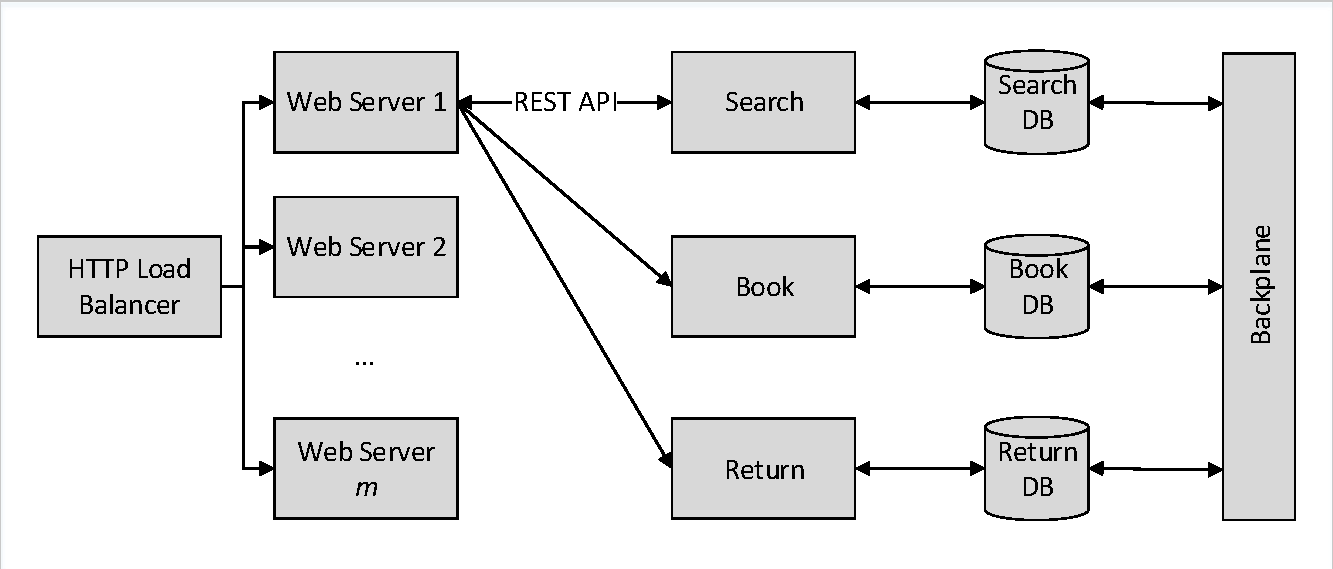
\includegraphics[trim = 5 5 5 5, clip, width=\textwidth]{img/microservices}
\end{figure}

\subsubsection{Evaluation.}
As for middleware, evaluation of different microservices approaches depends on end to end measurement.   However, one area of interest is the efficiency of highly granular microservices.  If the demand for the microservices is isolated then it is possible that some low demand services are underutilised.

%
% ---- Distributed databases
%

\subsection{Distributed databases}
Modern databases both SQL and NoSQL are designed to scale both data and the load of operations accessing that data over many servers that do not share disk or RAM, so-called ``shared nothing'' architecture \cite{RN67}.  We may partition data {\itshape vertically}, dividing tables into groups of columns that may be placed on different data nodes; or {\itshape horizontally}, where the split is by row \cite{RN68}. 

In our use case, the quantity of data does not approach the levels of ``Big Data'' applications.  We are interested in partitioning as a means of scaling the demand for that data.  Our ticketing system will not require a large number of columns and the three operations outlined do not have significantly different column requirements.  Horizontal partitioning is most relevant.  The partition key of a Ticket table may be the Ticket Type, the Date, or the seat Row.  Demand for tickets is likely to vary by each of these attributes.  An alternative partitioning strategy would be to on denormalised tables supporting the query, book and return operations.  The load on each data node would follow the demand for the data types and operations placed there.

The scalability of distributed databases usually comes at the price of a relaxed consistency model - so-called BASE (Basically Available, Soft state, Eventually Consistent) rather than ACID (Atomic, Consistent, Isolated, Durable) transactions.  In our ticketing system, eventual consistency is clearly sufficient for the return ticket scenario - returned tickets do not have to be made immediately available for booking.  Individual ticket bookings must exist on only one partition to prevent the same ticket being booked more than once.  Eventual consistency between search and book operations requires the customer to tolerate the concept of ``reservation'' of a ticket for a short period until a booking can be confirmed \cite{RN1071}\cite{RN67}.

Another issue to be aware of is {\itshape replication}.   Most distributed databases offer replication of data from one partition to another for availability.  In our use case, if a data node is overloaded by demand, the system may failover to a copy of the data on another data node, but this will just transfer the demand elsewhere.  If this is also the primary data node of an otherwise low demand data type, then it may be overwhelmed in turn.

Where the high demand is unknown in advance, we need an adaptive strategy.  Workload-aware clustering algorithms do exist for the placement of new data, e.g. \cite{RN63}, but our use case has a fixed set of tickets.  Re-placement of existing data onto different partitions would be likely to require many reads, writes and deletes.

\begin{figure}
\caption{Distributed database, without and with replication}
\centering
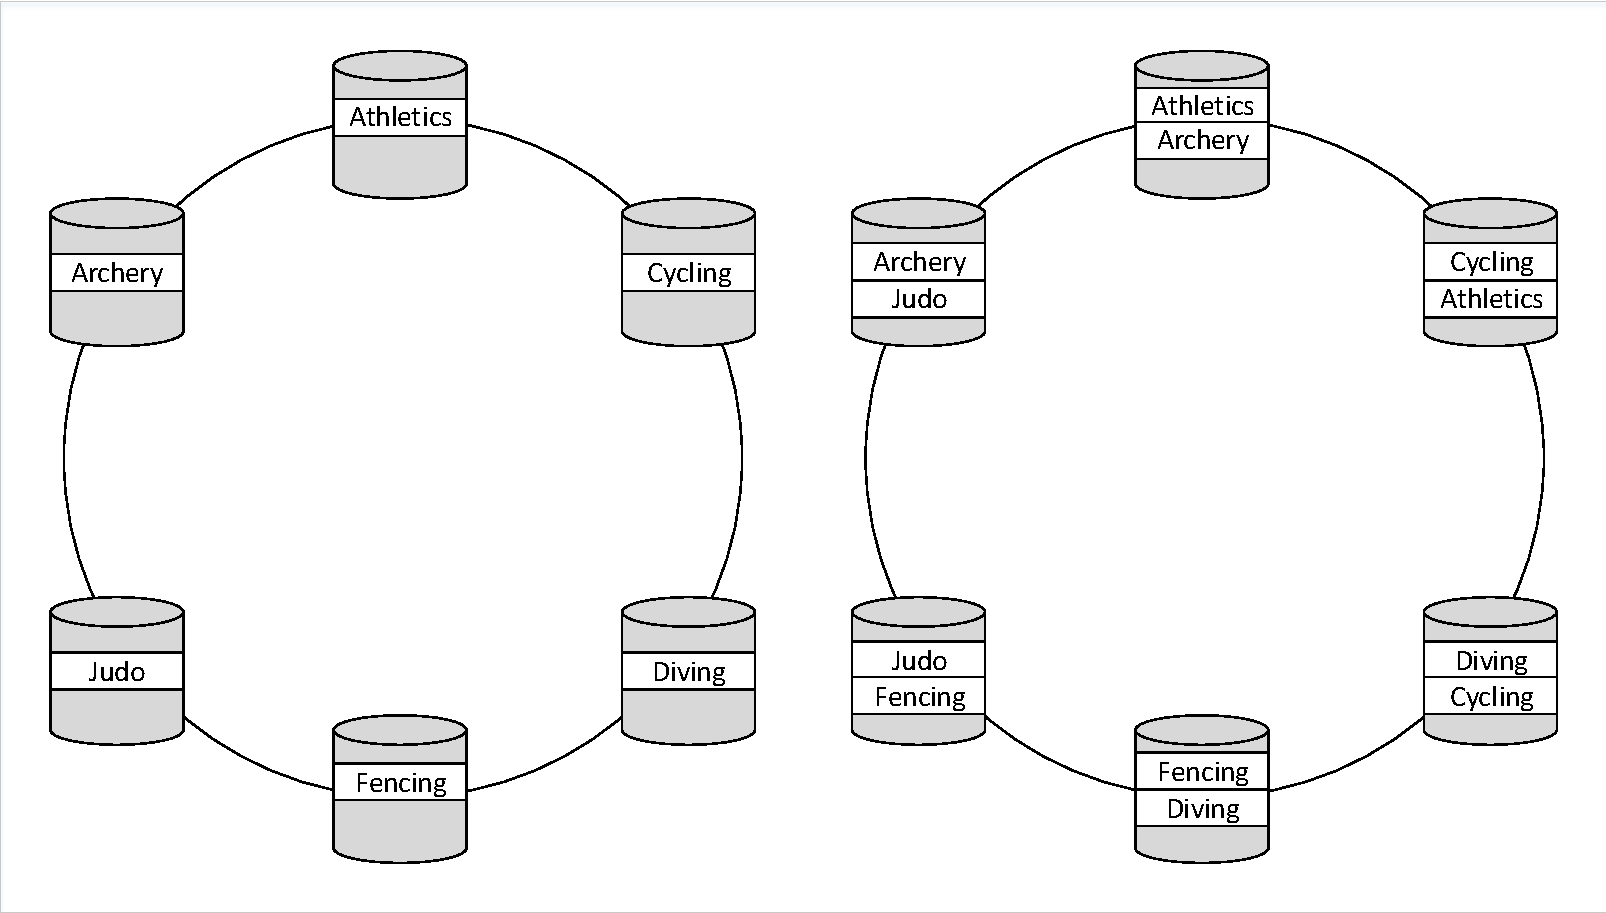
\includegraphics[trim = 5 5 5 5, clip, width=\textwidth]{img/dbdist}
\end{figure}

\subsubsection{Evaluation.}

A successful partitioning strategy will ensure that an individual operation only uses a single data node; that every data node is equally used when demand is evenly distributed; and that any impact from skewed demand is limited to the directly affected data node.

%
% ---- Modelling sub-document
%

\section{Modelling}

We can decouple worker applications from the front-end using asynchronous middleware.  Shared middleware balances the load, microservice architecture isolates it.  The system can adapt to current demand by using elastic scaling to create or destroy worker applications, and by using scaling groups we can ensure that the number of each application type is appropriate to the demand.

With care, we can use horizontal database partitioning to ensure that functions and/or data types are not shared between data nodes, isolating their demand from each other.

At the component level we can see whether an approach will balance or isolate load, or adapt to it, but at the system level we will need modelling techniques to predict the end to end throughput.

\paragraph{CloudSim.}  CloudSim \cite{calheiros2011cloudsim} is a Java framework for developing cloud datacentre simulations.  Much of it is concerned with modelling the efficient running of that infrastructure, for example the power usage, but it also includes utilisation models and may be useful for predicting the effect of elastic scaling.

CloudSim simulations require Java development for creation and modification, which is an overhead in building the models but offers more flexibility in applying them.  Process Algebra has closed-form solutions, though there is a PEPA Workbench tool \cite{gilmore1994pepa} that allows PEPA specifications to be parsed and run like programs, aiding experimentation on a range of action rates by automating repetitive calculations.  Both currently have their place as they predict different quantities of interest.

\paragraph{Process Algebra.} Process Algebras (such as PEPA or TIPP \cite{gotz1993multiprocessor}) allow us to model throughput in interdependent processes, with a mixture of independent and shared actions operating at different rates.  Each of our components can be described in this way, and queues have already been extensively modelled in PEPA \cite{thomas1997using}.  The nature of process algebra as a mathematical language also means that it is possible to build a model of a whole system by composition of the component models.

\begin{figure}
\caption{PEPA queue model}
\centering
% Automatically generated by PEPA2Latex
% --begin
\begin{displaymath}
	\begin{array}{rcl}
%[0.0ex]		
\mathit{Website} & \rmdef & (\mathit{request},\mathit{r}).\mathit{Website}\\
		\mathit{Worker} & \rmdef & (\mathit{service},\mathit{s}).\mathit{Worker}\\
		\mathit{Queue_{0}} & \rmdef & (\mathit{request},\mathit{r}).\mathit{Queue_{1}}\\
		\mathit{Queue_{1}} & \rmdef & (\mathit{service},\mathit{s}).\mathit{Queue_{0}}\\
[0.0ex]		\multicolumn{3}{l}{\mathit{Website}\sync{request}\mathit{Queue_{0}}[N]\sync{service}\mathit{Worker}}\\
[0.0ex]	\end{array}
\end{displaymath}
% --end
\end{figure}

%
% ---- PEPA Models
%

\section{PEPA Models}

%
% ---- Simple microservices
%
\subsection{Simple microservices}

\begin{figure}
	\caption{Simple microservices PEPA model}
	\centering
% --begin
\begin{displaymath}
	\begin{array}{rcl}
		\mathit{Website} & \rmdef & (\mathit{book\_athletics},\mathit{a}).\mathit{Website}+(\mathit{book\_cycling},\mathit{c}).\mathit{Website}\\
		\mathit{Athletics_{Worker}} & \rmdef & (\mathit{book\_athletics},\top).\mathit{Athletics_{Worker}}\\
		\mathit{Athletics_{DB}} & \rmdef & (\mathit{book\_athletics},\mathit{db\_a}).\mathit{Athletics_{DB}}\\
		\mathit{Cycling_{Worker}} & \rmdef & (\mathit{book\_cycling},\top).\mathit{Cycling_{Worker}}\\
		\mathit{Cycling_{DB}} & \rmdef & (\mathit{book\_cycling},\mathit{db\_c}).\mathit{Cycling_{DB}}\\
		[0.0ex]		\multicolumn{3}{l}{\mathit{Athletics_{Worker}}\sync{book\_athletics}\mathit{Website}\sync{book\_cycling}\mathit{Cycling_{Worker}}\sync{book\_athletics}\mathit{Athletics_{DB}}\sync{book\_cycling}\mathit{Cycling_{DB}}}\\
		[0.0ex]	\end{array}
\end{displaymath}
% --end
\end{figure}

\begin{figure}
	\caption{Simple microservices PEPA model - without worker processes}
	\centering
% --begin
\begin{displaymath}
\begin{array}{rcl}
		\mathit{Website} & \rmdef & (\mathit{book\_athletics},\mathit{a}).\mathit{Website}+(\mathit{book\_cycling},\mathit{c}).\mathit{Website}\\
\mathit{Athletics} & \rmdef & (\mathit{book\_athletics},\mathit{db\_a}).\mathit{Athletics}\\
\mathit{Cycling} & \rmdef & (\mathit{book\_cycling},\mathit{db\_c}).\mathit{Cycling}\\
[0.0ex]		\multicolumn{3}{l}{\mathit{Athletics}\sync{book\_athletics}\mathit{Website}\sync{book\_cycling}\mathit{Cycling}}\\
[0.0ex]	\end{array}
\end{displaymath}
% --end
\end{figure}

%
% ---- Operational microservices
%
\subsection{Operational microservices}



%
% ---- Shared queue middleware
%
\subsection{Shared queue middleware}

\begin{figure}
	\caption{Generic shared queue PEPA model}
	\centering
	% Automatically generated by PEPA2Latex
	% --begin
	\begin{displaymath}
		\begin{array}{rcl}
			\mathit{Arrival_1} & \rmdef & (\mathit{arrive_1},\mathit{a_1}).\mathit{Arrival_1}\\
			\mathit{Service_1} & \rmdef & (\mathit{serve_1},\mathit{s_1}).\mathit{Service_1}\\
			\mathit{Arrival_2} & \rmdef & (\mathit{arrive_2},\mathit{a_2}).\mathit{Arrival_2}\\
			\mathit{Service_2} & \rmdef & (\mathit{serve_2},\mathit{s_2}).\mathit{Service_2}\\
			\mathit{Q_0} & \rmdef & (\mathit{arrive_1},\top).\mathit{Q_1}+(\mathit{arrive_2},\top).\mathit{Q_1}\\
			\mathit{Q_1} & \rmdef & (\mathit{serve_1},\top).\mathit{Q_0}+(\mathit{serve_2},\top).\mathit{Q_0}\\
	[0.0ex]		\multicolumn{3}{l}{\mathit{Arrival_1}\sync{arrive_1}\mathit{Q_0}[N]\sync{serve_1}\mathit{Service_1}\sync{arrive_2}\mathit{Arrival_2}\sync{serve_2}\mathit{Service_2}}\\
	[0.0ex]	\end{array}
	\end{displaymath}
	% --end
\end{figure}

\begin{figure}
	\caption{Generic shared queue experimental results}
	\centering
	\begin{tikzpicture}
	\begin{axis}[
		title={Throughput of arrive\textsubscript{1} against input rate a\textsubscript{1} for different queue lengths N},
		xlabel={Rate a\textsubscript{1}},
		ylabel={Throughput arrive\textsubscript{1}},
		xmin=1, xmax=10,
		ymin=0, ymax=10,
		legend pos=north west,
		ymajorgrids=true,
		grid style=dashed,
		cycle multiindex* list={
			mark list*
				\nextlist
			cyan,brown,green,blue,red
		}
	]
	
	\addplot table [x index={0}, y index={1}, col sep=comma]{data/N1_arrive_1.csv};
	\addplot table [x index={0}, y index={1}, col sep=comma]{data/N2_arrive_1.csv};
	\addplot table [x index={0}, y index={1}, col sep=comma]{data/N5_arrive_1.csv};
	\addplot table [x index={0}, y index={1}, col sep=comma]{data/N10_arrive_1.csv};
	\addplot table [x index={0}, y index={1}, col sep=comma]{data/N20_arrive_1.csv};
	
	\legend{N = 1, N = 2, N = 5, N = 10, N = 20}

	\end{axis}
	\end{tikzpicture}
	
	\begin{tikzpicture}
	\begin{axis}[
	title={Throughput of serve\textsubscript{1} against input rate a\textsubscript{1} for different queue lengths N},
	xlabel={Rate a\textsubscript{1}},
	ylabel={Throughput serve\textsubscript{1}},
	xmin=1, xmax=10,
	ymin=0, ymax=5,
	legend pos=north west,
	ymajorgrids=true,
	grid style=dashed,
	cycle multiindex* list={
		mark list*
		\nextlist
		cyan,brown,green,blue,red
	}
	]
	
	\addplot table [x index={0}, y index={1}, col sep=comma]{data/N1_serve_1.csv};
	\addplot table [x index={0}, y index={1}, col sep=comma]{data/N2_serve_1.csv};
	\addplot table [x index={0}, y index={1}, col sep=comma]{data/N5_serve_1.csv};
	\addplot table [x index={0}, y index={1}, col sep=comma]{data/N10_serve_1.csv};
	\addplot table [x index={0}, y index={1}, col sep=comma]{data/N20_serve_1.csv};
	
	\legend{N = 1, N = 2, N = 5, N = 10, N = 20}
	
	\end{axis}
	\end{tikzpicture}
	
	\begin{tikzpicture}
	\begin{axis}[
	title={Throughput of arrive\textsubscript{2} against input rate a\textsubscript{1} for different queue lengths N},
	xlabel={Rate a\textsubscript{1}},
	ylabel={Throughput arrive\textsubscript{2}},
	xmin=1, xmax=10,
	ymin=0.4, ymax=1,
	legend pos=south west,
	ymajorgrids=true,
	grid style=dashed,
	cycle multiindex* list={
		mark list*
		\nextlist
		cyan,brown,green,blue,red
	}
	]
	
	\addplot table [x index={0}, y index={1}, col sep=comma]{data/N1_arrive_2.csv};
	\addplot table [x index={0}, y index={1}, col sep=comma]{data/N2_arrive_2.csv};
	\addplot table [x index={0}, y index={1}, col sep=comma]{data/N5_arrive_2.csv};
	\addplot table [x index={0}, y index={1}, col sep=comma]{data/N10_arrive_2.csv};
	\addplot table [x index={0}, y index={1}, col sep=comma]{data/N20_arrive_2.csv};
	
	\legend{N = 1, N = 2, N = 5, N = 10, N = 20}
	
	\end{axis}
	\end{tikzpicture}
\end{figure}

\begin{figure}
	\caption{Application specific shared queue PEPA model}
	\centering
	% --begin
	\begin{displaymath}
	\begin{array}{rcl}
	\mathit{Website} & \rmdef & (\mathit{book\_athletics},\mathit{a}).\mathit{Website}+(\mathit{book\_cycling},\mathit{c}).\mathit{Website}\\
	\mathit{Athletics_{arrival}} & \rmdef & (\mathit{book\_athletics},\top).\mathit{Athletics_{arrival}}\\
	\mathit{Cycling_{arrival}} & \rmdef & (\mathit{book\_cycling},\top).\mathit{Cycling_{arrival}}\\
	\mathit{DBnode_1} & \rmdef & (\mathit{book\_athletics\_db},\mathit{db\_1}).\mathit{DBnode_1}\\
	\mathit{DBnode_2} & \rmdef & (\mathit{book\_cycling\_db},\mathit{db\_2}).\mathit{DBnode_2}\\
	\mathit{Q_{empty}} & \rmdef & (\mathit{book\_athletics},\top).\mathit{Q_{athletics}}+(\mathit{book\_cycling},\top).\mathit{Q_{cycling}}\\
	\mathit{Q_{athletics}} & \rmdef & (\mathit{book\_athletics\_db},\top).\mathit{Q_{empty}}\\
	\mathit{Q_{cycling}} & \rmdef & (\mathit{book\_cycling\_db},\top).\mathit{Q_{empty}}\\
	[0.0ex]		\multicolumn{3}{l}{\mathit{Website}\sync{book\_athletics,book\_cycling}\mathit{Athletics_{arrival}}\sync{book\_athletics}\mathit{Q_{empty}}[N]\sync{book\_athletics\_db}\mathit{DBnode_1}\sync{book\_cycling}\mathit{Cycling_{arrival}}\sync{book\_cycling\_db}\mathit{DBnode_2}}\\
	[0.0ex]	\end{array}
	\end{displaymath}
	% --end
\end{figure}

\begin{figure}
	\caption{Shared queue PEPA model without queue arrival processes}
	\centering
	% --begin
	\begin{displaymath}
	\begin{array}{rcl}
	\mathit{Website} & \rmdef & (\mathit{book\_athletics},\mathit{a}).\mathit{Website}+(\mathit{book\_cycling},\mathit{c}).\mathit{Website}\\
	\mathit{DBnode_1} & \rmdef & (\mathit{book\_athletics\_db},\mathit{db\_1}).\mathit{DBnode_1}\\
	\mathit{DBnode_2} & \rmdef & (\mathit{book\_cycling\_db},\mathit{db\_2}).\mathit{DBnode_2}\\
	\mathit{Q_{empty}} & \rmdef & (\mathit{book\_athletics},\top).\mathit{Q_{athletics}}+(\mathit{book\_cycling},\top).\mathit{Q_{cycling}}\\
	\mathit{Q_{athletics}} & \rmdef & (\mathit{book\_athletics\_db},\top).\mathit{Q_{empty}}\\
	\mathit{Q_{cycling}} & \rmdef & (\mathit{book\_cycling\_db},\top).\mathit{Q_{empty}}\\
	[0.0ex]		\multicolumn{3}{l}{\mathit{Website}\sync{book\_athletics,book\_cycling}\mathit{Q_{empty}}[N]\sync{book\_athletics\_db}\mathit{DBnode_1}\sync{book\_cycling\_db}\mathit{DBnode_2}}\\
	[0.0ex]	\end{array}
	\end{displaymath}
	% --end
\end{figure}

%
% ---- Distributed database with replication
%
\subsection{Distributed database with replication}



%
% ---- Model components sub-document
%

%
% ---- PEPA Component Models
%

\section{PEPA Component Models}

%
% ---- Distributed database without replication
%
\subsection{Distributed database without replication}

The PEPA model for a distributed database is shown in Figure \ref{figure:pepa_dd_model}.

\begin{figure}
	\caption{Distributed database PEPA model}
	\label{figure:pepa_dd_model}
	\centering
	% Automatically generated by PEPA2Latex
	% --begin
	\begin{displaymath}
		\begin{array}{rcl}
			\mathit{Website} & \rmdef & (\mathit{book_a},\mathit{a}).\mathit{Website}+(\mathit{book_c},\mathit{c}).\mathit{Website}\\
			\mathit{DB_1} & \rmdef & (\mathit{book_a},\top).\mathit{DBsrv_1}\\
			\mathit{DBsrv_1} & \rmdef & (\mathit{dbsrv_1},\top).\mathit{DB_1}\\
			\mathit{DB_2} & \rmdef & (\mathit{book_c},\top).\mathit{DBsrv_2}\\
			\mathit{DBsrv_2} & \rmdef & (\mathit{dbsrv_2},\top).\mathit{DB_2}\\
			\mathit{Service_1} & \rmdef & (\mathit{dbsrv_1},\mathit{db}).\mathit{Service_1}\\
			\mathit{Service_2} & \rmdef & (\mathit{dbsrv_2},\mathit{db}).\mathit{Service_2}\\
	[0.0ex]		\multicolumn{3}{l}{\mathit{Website}\sync{book_a}\mathit{DB_1}\sync{book_c}\mathit{DB_2}\sync{dbsrv_1}\mathit{Service_1}\sync{dbsrv_2}\mathit{Service_2}}\\
	[0.0ex]	\end{array}
	\end{displaymath}
	% --end
\end{figure}

See the experimental results in Table \ref{table:dd_results}.

\begin{table}[h!]
	\begin{center}
		\caption{Distributed database experimental results}
		\label{table:dd_results}
			\pgfplotstabletypeset[
			col sep=comma,
			string type,
			columns/a/.style={column name=a, column type={p{.1\textwidth}}},
			columns/booka/.style={column name=book\textsubscript{a}, column type={p{.1\textwidth}}},
			columns/bookc/.style={column name=book\textsubscript{c}, column type={p{.1\textwidth}}},
			columns/dbsrv1/.style={column name=dbsrv\textsubscript{1}, column type={p{.1\textwidth}}},
			columns/dbsrv2/.style={column name=dbsrv\textsubscript{2}, column type={p{.1\textwidth}}},
			every head row/.style={before row=\hline Rate & \multicolumn{4}{c}{Throughput} \\,after row=\hline},
			every last row/.style={after row=\hline},
			]{data/ddnr/results.csv}
	\end{center}
\end{table}

\begin{figure}
	\caption{Distributed database experimental results}
	\label{figure:dd_charts}
	\centering
	\begin{tikzpicture}
	\begin{axis}[
		title={Throughput against input rate a},
		xlabel={Rate a},
		ylabel={Throughput},
		xmin=10, xmax=210,
		ymin=0, ymax=100,
		legend pos=north west,
		ymajorgrids=true,
		grid style=dashed,
		cycle multiindex* list={
			mark list*
				\nextlist
			cyan,brown,green,blue,red
		}
	]
	
	\addplot table [x index={0}, y index={1}, col sep=comma]{data/ddnr/book_a.csv};
	\addplot table [x index={0}, y index={1}, col sep=comma]{data/ddnr/book_c.csv};

	\legend{a,c}

	\end{axis}
	\end{tikzpicture}

	\begin{tikzpicture}
	\begin{axis}[
		title={Throughput against input rate a},
		xlabel={Rate a},
		ylabel={Throughput},
		xmin=10, xmax=210,
		ymin=0, ymax=100,
		legend pos=north west,
		ymajorgrids=true,
		grid style=dashed,
		cycle multiindex* list={
			mark list*
				\nextlist
			cyan,brown,green,blue,red
		}
	]
	
	\addplot table [x index={0}, y index={1}, col sep=comma]{data/ddnr/dbsrv_1.csv};
	\addplot table [x index={0}, y index={1}, col sep=comma]{data/ddnr/dbsrv_2.csv};

	\legend{dbsrv\textsubscript{1},dbsrv\textsubscript{2}}

	\end{axis}
	\end{tikzpicture}
\end{figure}

%
% ---- Distributed database with replication
%
\subsection{Distributed database with replication}

\begin{figure}
	\caption{Distributed database with replication PEPA model}
	\label{figure:pepa_ddwr_model}
	\centering
% Automatically generated by PEPA2Latex
% --begin
\begin{displaymath}
	\begin{array}{rcl}
		\mathit{Website} & \rmdef & (\mathit{book_a},\mathit{a}).\mathit{Website}+(\mathit{book_c},\mathit{c}).\mathit{Website}+(\mathit{book_d},\mathit{d}).\mathit{Website}\\
		\mathit{DB_1} & \rmdef & (\mathit{book_a},\top).\mathit{DBsrv_1}+(\mathit{book_c},\top).\mathit{DBsrv_1}\\
		\mathit{DBsrv_1} & \rmdef & (\mathit{dbsrv_1},\top).\mathit{DB_1}\\
		\mathit{DB_2} & \rmdef & (\mathit{book_c},\top).\mathit{DBsrv_2}+(\mathit{book_d},\top).\mathit{DBsrv_2}\\
		\mathit{DBsrv_2} & \rmdef & (\mathit{dbsrv_2},\top).\mathit{DB_2}\\
		\mathit{DB_3} & \rmdef & (\mathit{book_d},\top).\mathit{DBsrv_3}+(\mathit{book_a},\top).\mathit{DBsrv_3}\\
		\mathit{DBsrv_3} & \rmdef & (\mathit{dbsrv_3},\top).\mathit{DB_3}\\
		\mathit{Service_1} & \rmdef & (\mathit{dbsrv_1},\mathit{db}).\mathit{Service_1}\\
		\mathit{Service_2} & \rmdef & (\mathit{dbsrv_2},\mathit{db}).\mathit{Service_2}\\
		\mathit{Service_3} & \rmdef & (\mathit{dbsrv_3},\mathit{db}).\mathit{Service_3}\\
[0.0ex]		\multicolumn{3}{l}{\mathit{Website}\sync{book_a,book_c}\mathit{DB_1}\sync{book_c,book_d}\mathit{DB_2}\sync{book_d,book_a}\mathit{DB_3}\sync{dbsrv_1}\mathit{Service_1}\sync{dbsrv_2}\mathit{Service_2}\sync{dbsrv_3}\mathit{Service_3}}\\
[0.0ex]	\end{array}
\end{displaymath}
% --end
\end{figure}

See the experimental results in Table \ref{table:ddwr_results}.

\begin{table}[h!]
	\begin{center}
		\caption{Distributed database with replication experimental results}
		\label{table:ddwr_results}
		\pgfplotstabletypeset[
		col sep=comma,
		string type,
		columns/a/.style={column name=a, column type={p{.1\textwidth}}},
		columns/booka/.style={column name=book\textsubscript{a}, column type={p{.1\textwidth}}},
		columns/bookc/.style={column name=book\textsubscript{c}, column type={p{.1\textwidth}}},
		columns/bookd/.style={column name=book\textsubscript{d}, column type={p{.1\textwidth}}},
		columns/dbsrv1/.style={column name=dbsrv\textsubscript{1}, column type={p{.1\textwidth}}},
		columns/dbsrv2/.style={column name=dbsrv\textsubscript{2}, column type={p{.1\textwidth}}},
		columns/dbsrv3/.style={column name=dbsrv\textsubscript{3}, column type={p{.1\textwidth}}},
		every head row/.style={before row=\hline Rate & \multicolumn{6}{c}{Throughput} \\,after row=\hline},
		every last row/.style={after row=\hline},
		]{data/ddwr/results.csv}
	\end{center}
\end{table}

\begin{figure}
	\caption{Distributed database with replication experimental results}
	\label{figure:ddwr_charts}
	\centering
	\begin{tikzpicture}
	\begin{axis}[
		title={Throughput against input rate a},
		xlabel={Rate a},
		ylabel={Throughput},
		xmin=10, xmax=210,
		ymin=0, ymax=100,
		legend pos=north west,
		ymajorgrids=true,
		grid style=dashed,
		cycle multiindex* list={
			mark list*
				\nextlist
			cyan,brown,green,blue,red
		}
	]
	
	\addplot table [x index={0}, y index={1}, col sep=comma]{data/ddwr/book_a.csv};
	\addplot table [x index={0}, y index={1}, col sep=comma]{data/ddwr/book_c.csv};
	\addplot table [x index={0}, y index={1}, col sep=comma]{data/ddwr/book_d.csv};

	\legend{a,c,d}

	\end{axis}
	\end{tikzpicture}

	\begin{tikzpicture}
	\begin{axis}[
		title={Throughput against input rate a},
		xlabel={Rate a},
		ylabel={Throughput},
		xmin=10, xmax=210,
		ymin=0, ymax=100,
		legend pos=north west,
		ymajorgrids=true,
		grid style=dashed,
		cycle multiindex* list={
			mark list*
				\nextlist
			cyan,brown,green,blue,red
		}
	]
	
	\addplot table [x index={0}, y index={1}, col sep=comma]{data/ddwr/dbsrv_1.csv};
	\addplot table [x index={0}, y index={1}, col sep=comma]{data/ddwr/dbsrv_2.csv};
	\addplot table [x index={0}, y index={1}, col sep=comma]{data/ddwr/dbsrv_3.csv};

	\legend{dbsrv\textsubscript{1},dbsrv\textsubscript{2},dbsrv\textsubscript{3}}

	\end{axis}
	\end{tikzpicture}
\end{figure}

%
% ---- Shared middleware queue
%
\subsection{Shared middleware queue}

\begin{figure}
	\caption{Generic shared queue PEPA model}
	\label{figure:pepa_queue_model}
	\centering
	% Automatically generated by PEPA2Latex
	% --begin
	\begin{displaymath}
		\begin{array}{rcl}
			\mathit{Arrival_1} & \rmdef & (\mathit{arrive_1},\mathit{a_1}).\mathit{Arrival_1}\\
			\mathit{Service_1} & \rmdef & (\mathit{serve_1},\mathit{s_1}).\mathit{Service_1}\\
			\mathit{Arrival_2} & \rmdef & (\mathit{arrive_2},\mathit{a_2}).\mathit{Arrival_2}\\
			\mathit{Service_2} & \rmdef & (\mathit{serve_2},\mathit{s_2}).\mathit{Service_2}\\
			\mathit{Q_0} & \rmdef & (\mathit{arrive_1},\top).\mathit{Q_1}+(\mathit{arrive_2},\top).\mathit{Q_1}\\
			\mathit{Q_1} & \rmdef & (\mathit{serve_1},\top).\mathit{Q_0}+(\mathit{serve_2},\top).\mathit{Q_0}\\
	[0.0ex]		\multicolumn{3}{l}{\mathit{Arrival_1}\sync{arrive_1}\mathit{Q_0}[N]\sync{serve_1}\mathit{Service_1}\sync{arrive_2}\mathit{Arrival_2}\sync{serve_2}\mathit{Service_2}}\\
	[0.0ex]	\end{array}
	\end{displaymath}
	% --end
\end{figure}

\begin{figure}
	\caption{Generic shared queue experimental results}
	\label{figure:queue_charts}
	\centering
	\begin{tikzpicture}
	\begin{axis}[
		title={Throughput of arrive\textsubscript{1} against input rate a\textsubscript{1} for different queue lengths N},
		xlabel={Rate a\textsubscript{1}},
		ylabel={Throughput arrive\textsubscript{1}},
		xmin=1, xmax=10,
		ymin=0, ymax=10,
		legend pos=north west,
		ymajorgrids=true,
		grid style=dashed,
		cycle multiindex* list={
			mark list*
				\nextlist
			cyan,brown,green,blue,red
		}
	]
	
	\addplot table [x index={0}, y index={1}, col sep=comma]{data/N1_arrive_1.csv};
	\addplot table [x index={0}, y index={1}, col sep=comma]{data/N2_arrive_1.csv};
	\addplot table [x index={0}, y index={1}, col sep=comma]{data/N5_arrive_1.csv};
	\addplot table [x index={0}, y index={1}, col sep=comma]{data/N10_arrive_1.csv};
	\addplot table [x index={0}, y index={1}, col sep=comma]{data/N20_arrive_1.csv};
	
	\legend{N = 1, N = 2, N = 5, N = 10, N = 20}

	\end{axis}
	\end{tikzpicture}
	
	\begin{tikzpicture}
	\begin{axis}[
	title={Throughput of serve\textsubscript{1} against input rate a\textsubscript{1} for different queue lengths N},
	xlabel={Rate a\textsubscript{1}},
	ylabel={Throughput serve\textsubscript{1}},
	xmin=1, xmax=10,
	ymin=0, ymax=5,
	legend pos=north west,
	ymajorgrids=true,
	grid style=dashed,
	cycle multiindex* list={
		mark list*
		\nextlist
		cyan,brown,green,blue,red
	}
	]
	
	\addplot table [x index={0}, y index={1}, col sep=comma]{data/N1_serve_1.csv};
	\addplot table [x index={0}, y index={1}, col sep=comma]{data/N2_serve_1.csv};
	\addplot table [x index={0}, y index={1}, col sep=comma]{data/N5_serve_1.csv};
	\addplot table [x index={0}, y index={1}, col sep=comma]{data/N10_serve_1.csv};
	\addplot table [x index={0}, y index={1}, col sep=comma]{data/N20_serve_1.csv};
	
	\legend{N = 1, N = 2, N = 5, N = 10, N = 20}
	
	\end{axis}
	\end{tikzpicture}
	
	\begin{tikzpicture}
	\begin{axis}[
	title={Throughput of arrive\textsubscript{2} against input rate a\textsubscript{1} for different queue lengths N},
	xlabel={Rate a\textsubscript{1}},
	ylabel={Throughput arrive\textsubscript{2}},
	xmin=1, xmax=10,
	ymin=0.4, ymax=1,
	legend pos=south west,
	ymajorgrids=true,
	grid style=dashed,
	cycle multiindex* list={
		mark list*
		\nextlist
		cyan,brown,green,blue,red
	}
	]
	
	\addplot table [x index={0}, y index={1}, col sep=comma]{data/N1_arrive_2.csv};
	\addplot table [x index={0}, y index={1}, col sep=comma]{data/N2_arrive_2.csv};
	\addplot table [x index={0}, y index={1}, col sep=comma]{data/N5_arrive_2.csv};
	\addplot table [x index={0}, y index={1}, col sep=comma]{data/N10_arrive_2.csv};
	\addplot table [x index={0}, y index={1}, col sep=comma]{data/N20_arrive_2.csv};
	
	\legend{N = 1, N = 2, N = 5, N = 10, N = 20}
	
	\end{axis}
	\end{tikzpicture}
\end{figure}

%
% ---- Model system sub-document
%

%
% ---- PEPA System Models
%

\section{PEPA System Models}\label{sec:pepa-system-models}
\begin{shaded}
The proposed system will use distributed architectures.  Users will access it from a web-based front end.  Tickets will be stored in a database partitioned across several data nodes.  In between the web servers and database will be a number of worker applications to service user requests, connected to the web servers by some middleware.

For each architecture it will be assumed that the web application will be designed to cope with the required demand, using a cluster of web servers where the throughput is managed using some HTTP Load Balancing algorithm \cite{RN73}, and potentially Elastic Scaling of servers e.g. using the autoscaling features of Amazon Web Services \cite{RN1064} or Microsoft Azure \cite{RN1065}.
\end{shaded}

%
% ---- Simple microservices
%
\subsection{Simple microservices}

There are two separate databases, one for Athletics tickets, one for Cycling.

It's expected that this architecture will lead to isolation of the skewed demand and that the results of testing the model will not be surprising, but that this will provide a useful control for other architectures.

\begin{figure}
	\caption{Simple microservices architecture}
	\centering
	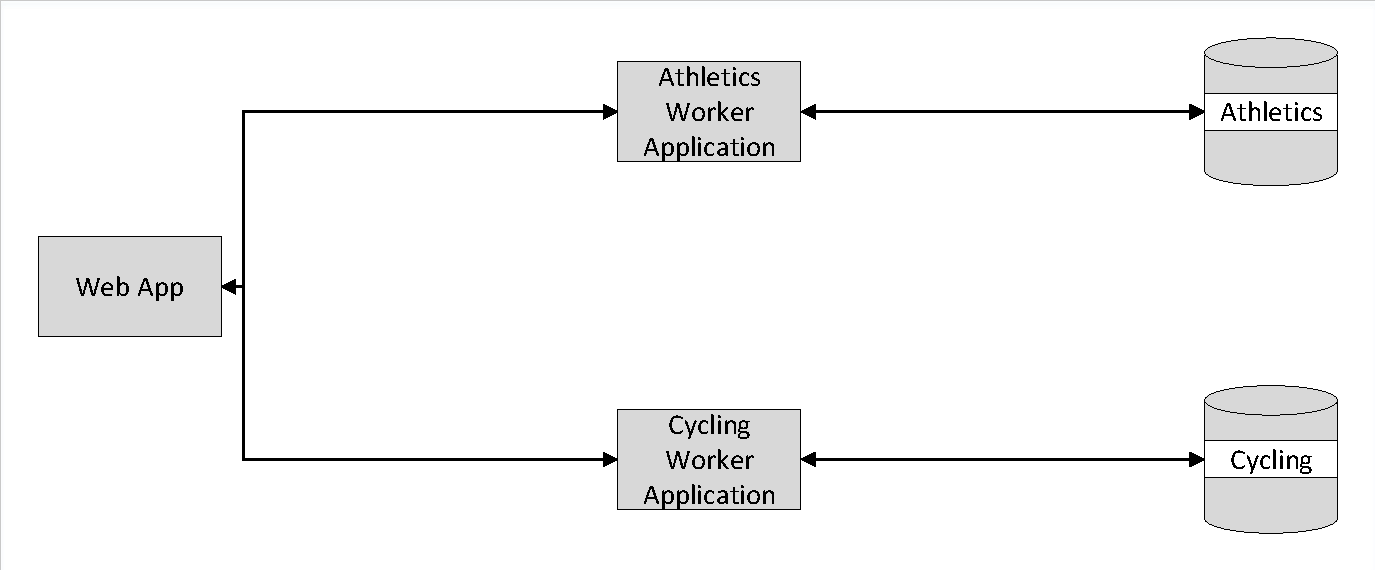
\includegraphics[trim = 5 5 5 5, clip, width=\textwidth]{img/simplemicro}
\end{figure}

\begin{figure}
	\caption{Simple microservices PEPA model}
	\label{figure:simplemicro}
	\centering
	% Automatically generated by PEPA2Latex
	% --begin
	\begin{displaymath}
		\begin{array}{rcl}
			\mathit{a} & = & 1.0 - 10.0\\
			\mathit{c} & = & 1.0\\
			\mathit{w} & = & 100.0\\
			\mathit{db} & = & 6.5\\
			[2.0ex]		\mathit{Website} & \rmdef & (\mathit{athletics},\mathit{a}).\mathit{Website}+(\mathit{cycling},\mathit{c}).\mathit{Website}\\
			\mathit{Worker_A} & \rmdef & (\mathit{athletics},\top).\mathit{WorkerSrv_A}\\
			\mathit{WorkerSrv_A} & \rmdef & (\mathit{workerA},\top).\mathit{Worker_A}\\
			\mathit{Worker_C} & \rmdef & (\mathit{cycling},\top).\mathit{WorkerSrv_C}\\
			\mathit{WorkerSrv_C} & \rmdef & (\mathit{workerC},\top).\mathit{Worker_C}\\
			\mathit{DB_1} & \rmdef & (\mathit{workerA},\mathit{w}).\mathit{DBsrv_1}\\
			\mathit{DBsrv_1} & \rmdef & (\mathit{dbsrv1},\mathit{db}).\mathit{DB_1}\\
			\mathit{DB_2} & \rmdef & (\mathit{workerC},\mathit{w}).\mathit{DBsrv_2}\\
			\mathit{DBsrv_2} & \rmdef & (\mathit{dbsrv2},\mathit{db}).\mathit{DB_2}\\
			\mathit{Service_1} & \rmdef & (\mathit{dbsrv1},\mathit{db}).\mathit{Service_1}\\
			\mathit{Service_2} & \rmdef & (\mathit{dbsrv2},\mathit{db}).\mathit{Service_2}\\
			[2.0ex]		\multicolumn{3}{l}{\mathit{Service_1}\sync{dbsrv1}\mathit{DB_1}\sync{workerA}\mathit{Worker_A}\sync{athletics}\mathit{Website}\sync{cycling}\mathit{Worker_C}\sync{workerC}\mathit{DB_2}\sync{dbsrv2}\mathit{Service_2}}\\
			[2.0ex]	\end{array}
	\end{displaymath}
	% --end
\end{figure}

See the experimental results in Table \ref{table:micro_results}.

\begin{table}[h!]
	\begin{center}
		\caption{Simple microservices experimental results}
		\label{table:micro_results}
		\pgfplotstabletypeset[
		col sep=comma,
		string type,
		columns/a/.style={column name=a, column type={p{.1\textwidth}}},
		columns/athletics/.style={column name=athletics, column type={p{.1\textwidth}}},
		columns/cycling/.style={column name=cycling, column type={p{.1\textwidth}}},
		columns/workerA/.style={column name=workerA, column type={p{.1\textwidth}}},
		columns/workerC/.style={column name=workerC, column type={p{.1\textwidth}}},
		columns/dbsrv1/.style={column name=dbsrv1, column type={p{.1\textwidth}}},
		columns/dbsrv2/.style={column name=dbsrv2, column type={p{.1\textwidth}}},
		every head row/.style={before row=\hline Rate & \multicolumn{6}{c}{Throughput} \\,after row=\hline},
		every last row/.style={after row=\hline},
		]{data/micro/results.csv}
	\end{center}
\end{table}

\begin{figure}
	\caption{Simple microservices experimental results}
	\label{figure:micro_charts}
	\centering
	\begin{tikzpicture}
	\begin{axis}[
	title={Throughput against input rate a},
	xlabel={Rate a},
	ylabel={Throughput},
	xmin=0, xmax=10,
	ymin=0, ymax=7,
	legend pos=north west,
	ymajorgrids=true,
	grid style=dashed,
	cycle multiindex* list={
		mark list*
		\nextlist
		cyan,brown,green,blue,red
	}
	]
	
	\addplot table [x index={0}, y index={1}, col sep=comma]{data/micro/athletics.csv};
	\addplot table [x index={0}, y index={1}, col sep=comma]{data/micro/cycling.csv};
	
	\legend{athletics,cycling}
	
	\end{axis}
	\end{tikzpicture}
\end{figure}

%
% ---- Shared queue and distributed database
%
\subsection{Shared queue and distributed database}

Requests via a shared queue to worker applications going to a distributed database with two nodes, Athletics and Cycling.

\begin{figure}
	\caption{Shared queue middleware architecture}
	\centering
	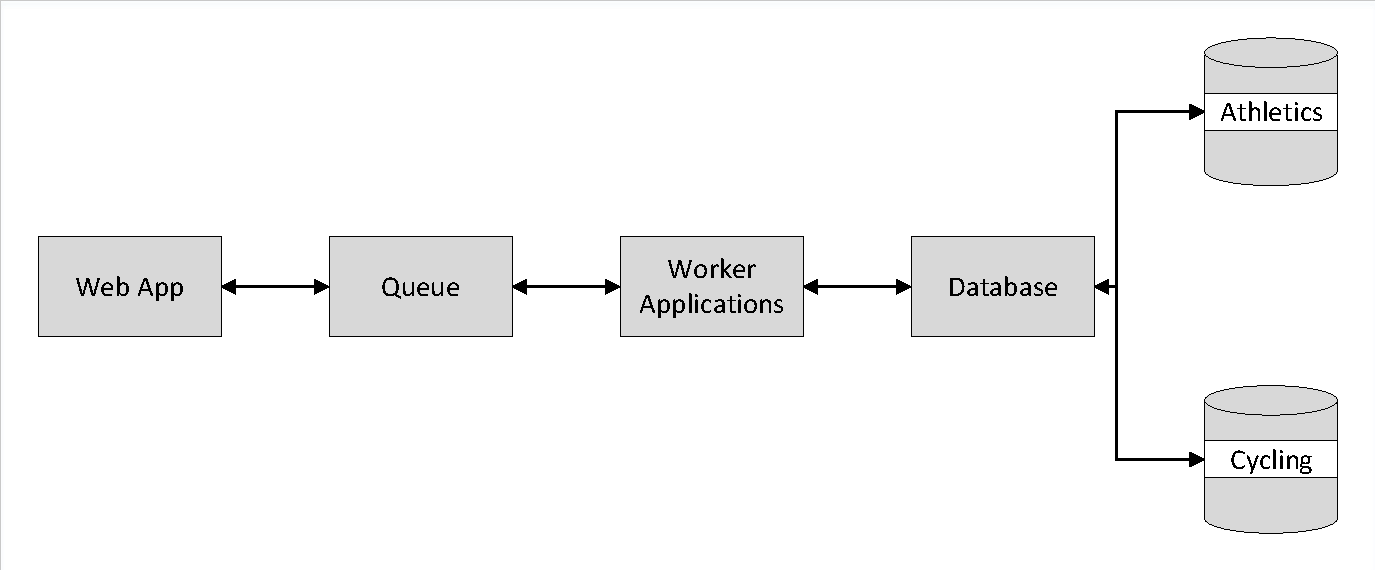
\includegraphics[trim = 5 5 5 5, clip, width=\textwidth]{img/sharedqueue}
\end{figure}

\begin{figure}
	\caption{Shared queue and distributed database}
	\label{figure:queuedd}
	\centering
	% Automatically generated by PEPA2Latex
	% --begin
	\begin{displaymath}
	\begin{array}{rcl}
	\mathit{a} & = & 1.0\\
	\mathit{c} & = & 1.0\\
	\mathit{q} & = & 100.0\\
	\mathit{db} & = & 5.0\\
	[2.0ex]		\mathit{Website} & \rmdef & (\mathit{athletics},\mathit{a}).\mathit{Website}+(\mathit{cycling},\mathit{c}).\mathit{Website}\\
	\mathit{Q_0} & \rmdef & (\mathit{athletics},\top).\mathit{Q_A}+(\mathit{cycling},\top).\mathit{Q_C}\\
	\mathit{Q_A} & \rmdef & (\mathit{queueA},\top).\mathit{Q_0}\\
	\mathit{Q_C} & \rmdef & (\mathit{queueC},\top).\mathit{Q_0}\\
	\mathit{DB_1} & \rmdef & (\mathit{queueA},\mathit{q}).\mathit{DBsrv_1}\\
	\mathit{DBsrv_1} & \rmdef & (\mathit{dbsrv1},\mathit{db}).\mathit{DB_1}\\
	\mathit{DB_2} & \rmdef & (\mathit{queueC},\mathit{q}).\mathit{DBsrv_2}\\
	\mathit{DBsrv_2} & \rmdef & (\mathit{dbsrv2},\mathit{db}).\mathit{DB_2}\\
	\mathit{Service_1} & \rmdef & (\mathit{dbsrv1},\mathit{db}).\mathit{Service_1}\\
	\mathit{Service_2} & \rmdef & (\mathit{dbsrv2},\mathit{db}).\mathit{Service_2}\\
	[2.0ex]		\multicolumn{3}{l}{\mathit{Website}\sync{\substack{athletics\\cycling}}\mathit{Q_0}[10]\sync{\substack{queueA\\queueC}}\mathit{DB_1}\parallel\mathit{DB_2}\sync{\substack{dbsrv1\\dbsrv2}}\mathit{Service_1}\parallel\mathit{Service_2}}\\
	[2.0ex]	\end{array}
	\end{displaymath}
	% --end
\end{figure}

See the experimental results in Table \ref{table:queuedd_results}.

\begin{table}[h!]
	\begin{center}
		\caption{Shared queue and distributed database experimental results}
		\label{table:queuedd_results}
		\pgfplotstabletypeset[
		col sep=comma,
		string type,
		columns/a/.style={column name=a, column type={p{.1\textwidth}}},
		columns/athletics/.style={column name=athletics, column type={p{.1\textwidth}}},
		columns/cycling/.style={column name=cycling, column type={p{.1\textwidth}}},
		columns/qa/.style={column name=queueA, column type={p{.1\textwidth}}},
		columns/qc/.style={column name=queueC, column type={p{.1\textwidth}}},
		columns/dbsrv1/.style={column name=dbsrv1, column type={p{.1\textwidth}}},
		columns/dbsrv2/.style={column name=dbsrv2, column type={p{.1\textwidth}}},
		every head row/.style={before row=\hline Rate & \multicolumn{6}{c}{Throughput} \\,after row=\hline},
		every last row/.style={after row=\hline},
		]{data/qddnr/results.csv}
	\end{center}
\end{table}

%
% ---- Shared queue and distributed database with replication
%
\subsection{Shared queue and distributed database with replication}

Requests via a shared queue to worker applications going to a distributed database with three nodes, Athletics, Cycling and Diving, where each partition is replicated on another node.

\begin{figure}
	\caption{Distributed database with replication architecture}
	\centering
	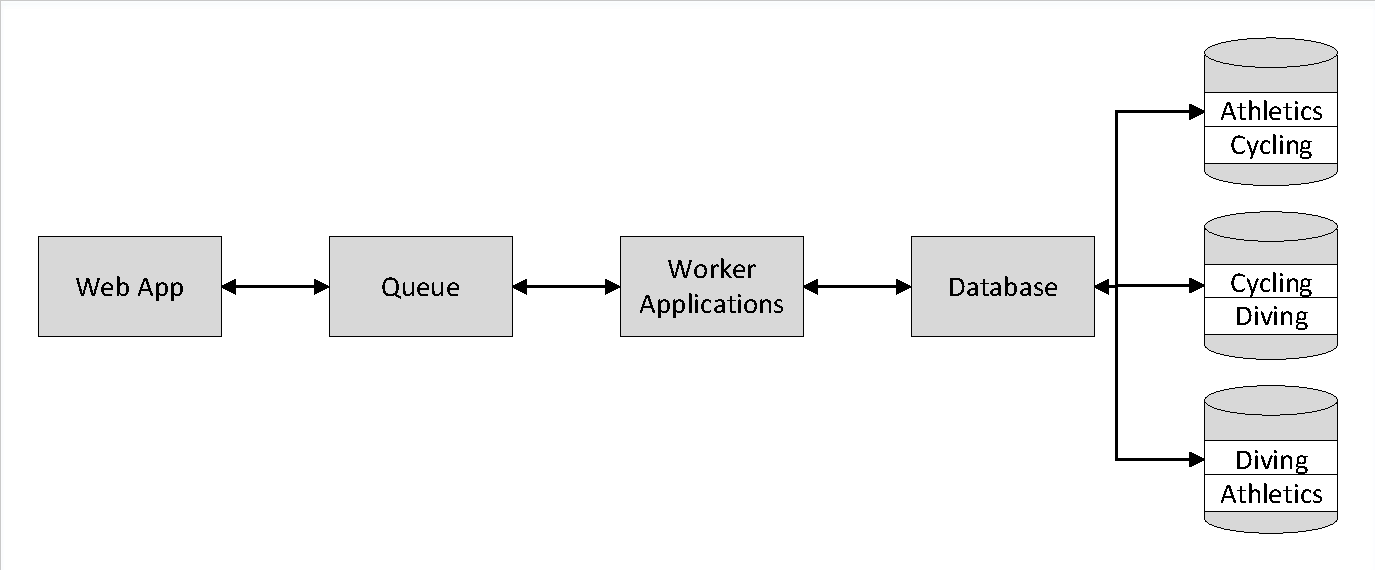
\includegraphics[trim = 5 5 5 5, clip, width=\textwidth]{img/sharedqueue_withrep}
\end{figure}

\begin{figure}
	\caption{Shared queue and distributed database with replication}
	\label{figure:queueddrep}
	\centering
	% Automatically generated by PEPA2Latex
	% --begin
	\begin{displaymath}
	\begin{array}{rcl}
	\mathit{a} & = & 1.0\\
	\mathit{c} & = & 1.0\\
	\mathit{d} & = & 1.0\\
	\mathit{q} & = & 100.0\\
	\mathit{db} & = & 5.0\\
	[2.0ex]		\mathit{Website} & \rmdef & (\mathit{athletics},\mathit{a}).\mathit{Website}+(\mathit{cycling},\mathit{c}).\mathit{Website}+(\mathit{diving},\mathit{d}).\mathit{Website}\\
	\mathit{Q_0} & \rmdef & (\mathit{athletics},\top).\mathit{Q_A}+(\mathit{cycling},\top).\mathit{Q_C}+(\mathit{diving},\top).\mathit{Q_D}\\
	\mathit{Q_A} & \rmdef & (\mathit{queueA},\top).\mathit{Q_0}\\
	\mathit{Q_C} & \rmdef & (\mathit{queueC},\top).\mathit{Q_0}\\
	\mathit{Q_D} & \rmdef & (\mathit{queueD},\top).\mathit{Q_0}\\
	\mathit{DB_1} & \rmdef & (\mathit{queueA},\mathit{q}).\mathit{DBsrv_1}+(\mathit{queueC},\mathit{q}).\mathit{DBsrv_1}\\
	\mathit{DBsrv_1} & \rmdef & (\mathit{dbsrv1},\top).\mathit{DB_1}\\
	\mathit{DB_2} & \rmdef & (\mathit{queueC},\mathit{q}).\mathit{DBsrv_2}+(\mathit{queueD},\mathit{q}).\mathit{DBsrv_2}\\
	\mathit{DBsrv_2} & \rmdef & (\mathit{dbsrv2},\top).\mathit{DB_2}\\
	\mathit{DB_3} & \rmdef & (\mathit{queueD},\mathit{q}).\mathit{DBsrv_3}+(\mathit{queueA},\mathit{q}).\mathit{DBsrv_3}\\
	\mathit{DBsrv_3} & \rmdef & (\mathit{dbsrv3},\top).\mathit{DB_3}\\
	\mathit{Service_1} & \rmdef & (\mathit{dbsrv1},\mathit{db}).\mathit{Service_1}\\
	\mathit{Service_2} & \rmdef & (\mathit{dbsrv2},\mathit{db}).\mathit{Service_2}\\
	\mathit{Service_3} & \rmdef & (\mathit{dbsrv3},\mathit{db}).\mathit{Service_3}\\
	[2.0ex]		\multicolumn{3}{l}{\mathit{Website}\sync{\substack{athletics\\cycling\\diving}}\mathit{Q_0}[10]\sync{\substack{queueA\\queueC\\queueD}}\mathit{DB_1}\parallel\mathit{DB_2}\parallel\mathit{DB_3}\sync{\substack{dbsrv1\\dbsrv2\\dbsrv3}}\mathit{Service_1}\parallel\mathit{Service_2}\parallel\mathit{Service_3}}\\
	[2.0ex]	\end{array}
	\end{displaymath}
	% --end
\end{figure}

See the experimental results in Table \ref{table:queueddwr_results}.

\begin{table}[h!]
	\begin{center}
		\caption{Shared queue and distributed database with replication experimental results}
		\label{table:queueddwr_results}
		\pgfplotstabletypeset[
		col sep=comma,
		string type,
		columns/a/.style={column name=a, column type={p{.1\textwidth}}},
		columns/athletics/.style={column name=athletics, column type={p{.1\textwidth}}},
		columns/cycling/.style={column name=cycling, column type={p{.1\textwidth}}},
		columns/diving/.style={column name=diving, column type={p{.1\textwidth}}},
		columns/qa/.style={column name=queueA, column type={p{.1\textwidth}}},
		columns/qc/.style={column name=queueC, column type={p{.1\textwidth}}},
		columns/qd/.style={column name=queueD, column type={p{.1\textwidth}}},
		columns/dbsrv1/.style={column name=dbsrv1, column type={p{.1\textwidth}}},
		columns/dbsrv2/.style={column name=dbsrv2, column type={p{.1\textwidth}}},
		columns/dbsrv3/.style={column name=dbsrv3, column type={p{.1\textwidth}}},
		every head row/.style={before row=\hline Rate & \multicolumn{9}{c}{Throughput} \\,after row=\hline},
		every last row/.style={after row=\hline},
		]{data/qddwr/results.csv}
	\end{center}
\end{table}

%
% ---- System comparison
%
\subsection{Comparison}

\begin{shaded}
The system results are compared in Table \ref{table:comparison_results}.

This shows that the simple microservices system does a good job of isolating the skewed demand from the rest of the system, but it is an inefficient use of the database resources.  The actual throughput of the athletics demand is limited to its database's throughput, while the spare capacity of the cycling database goes unused.  Using a distributed database with replication by contrast uses the capacity of two database nodes to serve the skewed demand, so that the actual throughput is much closer to the desired value.

(NOTE: the replication model uses 3 nodes, the others use 2 - need to compare like with like.  Try all with 3 or replication with 2?)
\end{shaded}

\begin{table}[h!]
	\begin{center}
		\caption{Comparison of system results}
		\label{table:comparison_results}
		\pgfplotstabletypeset[
		col sep=comma,
		string type,
		columns/a/.style={column name=a, column type={p{.1\textwidth}}},
		columns/amicro/.style={column name=athletics, column type={p{.15\textwidth}}},
		columns/cmicro/.style={column name=cycling, column type={p{.15\textwidth}}},
		columns/aqddnr/.style={column name=athletics, column type={p{.15\textwidth}}},
		columns/cqddnr/.style={column name=cycling, column type={p{.15\textwidth}}},
		columns/aqddwr/.style={column name=athletics, column type={p{.15\textwidth}}},
		columns/cqddwr/.style={column name=cycling, column type={p{.15\textwidth}}},
		every head row/.style={before row=\hline Rate & \multicolumn{2}{l}{Microservices} & \multicolumn{2}{l}{Queue + Distributed DB} & \multicolumn{2}{l}{Queue + DB with Replication} \\,after row=\hline},
		every last row/.style={after row=\hline},
		]{data/compare.csv}
	\end{center}
\end{table}

\begin{figure}
	\caption{Simple microservices experimental results}
	\label{figure:comparison_charts}
	\centering
	\begin{tikzpicture}
	\begin{axis}[
	title={Throughput of athletics against input rate a},
	width=0.9\textwidth,
	xlabel={Rate a},
	ylabel={Throughput},
	xmin=0, xmax=10,
	ymin=0, ymax=10,
	legend pos=north west,
	legend cell align={left},
	ymajorgrids=true,
	grid style=dashed,
	cycle multiindex* list={
		mark list*
		\nextlist
		cyan,brown,green,blue,red
	}
	]
	
	\addplot table [x index={0}, y index={1}, col sep=comma]{data/micro/athletics.csv};
	\addplot table [x index={0}, y index={1}, col sep=comma]{data/qddnr/athletics.csv};
	\addplot table [x index={0}, y index={1}, col sep=comma]{data/qddwr/athletics.csv};
	
	\legend{Simple Microservices,Queue + Distributed DB,Queue + Distributed DB with Replication}
	
	\end{axis}
	\end{tikzpicture}
	
		\begin{tikzpicture}
	\begin{axis}[
	title={Throughput of cycling against input rate a},
	width=0.9\textwidth,
	xlabel={Rate a},
	ylabel={Throughput},
	xmin=0, xmax=10,
	ymin=0, ymax=1.2,
	legend pos=south west,
	legend cell align={left},
	ymajorgrids=true,
	grid style=dashed,
	cycle multiindex* list={
		mark list*
		\nextlist
		cyan,brown,green,blue,red
	}
	]
	
	\addplot table [x index={0}, y index={1}, col sep=comma]{data/micro/cycling.csv};
	\addplot table [x index={0}, y index={1}, col sep=comma]{data/qddnr/cycling.csv};
	\addplot table [x index={0}, y index={1}, col sep=comma]{data/qddwr/cycling.csv};
	
	\legend{Simple Microservices,Queue + Distributed DB,Queue + Distributed DB with Replication}
	
	\end{axis}
	\end{tikzpicture}
\end{figure}

%
% ---- Built systems sub-document
%

%
% ---- Built systems
%

\section{Built systems}

Reference to github at \cite{RN1073}

General design decisions:

Cassandra \cite{RN1050}\cite{RN1075} database.

Measurement using Coda Hale Metrics \cite{RN1079}.

Load testing using Apache JMeter \cite{RN1074}.

%
% ---- Simple microservices
%
\subsection{Simple microservices}

RESTful APIs using Java Spring \cite{RN1076}.

%
% ---- Shared queue middleware
%
\subsection{Shared queue middleware}

%
% ---- Distributed database with replication
%
\subsection{Distributed database with replication}



%
% ---- Conclusion sub-document
%

\section{Conclusion and Future Work}
In this article we showed that cloud technologies could manipulate the throughput at each of the layers of our ticketing system architecture.
\paragraph{Front-end.}  We can balance demand at the web front-end using content-blind HTTP load balancing, and isolate skewed demand using content-aware algorithms.  Elastic scaling of web servers enables the front-end to respond to as much demand as the system owner is willing to pay for.
\paragraph{Application.} We can decouple worker applications from the front-end using asynchronous middleware.  Shared middleware balances the load, microservice architecture isolates it.  The system can adapt to current demand by using elastic scaling to create or destroy worker applications, and by using scaling groups we can ensure that the number of each application type is appropriate to the demand.
\paragraph{Database.} With care, we can use horizontal database partitioning to ensure that functions and/or data types are not shared between data nodes, isolating their demand from each other.

At the component level we can see whether an approach will balance or isolate load, or adapt to it, but at the system level we will need modelling techniques to predict the end to end throughput.  We looked at two approaches, process algebra and programmatic, that could be used to build complex models from smaller components.

An interesting area of future work would be to create a test system based on Red Hat's Ticket Monster application \cite{redhatticketmonster} and build it both as a model in PEPA, and an instrumented system running alongside it on real infrastructure. The model's predictions could then be tested against measurements of the real system.  Both model and real system could be deployed in different configurations of interest - balancing demand via shared middleware or isolating it via the microservices approach - to see how each copes with different demand scenarios.  For example, with rising skewed demand for one ticket type, at what point does the balanced demand approach begin to affect the entire system?  Do either of the shared middleware and microservices approaches have clear efficiency advantages under certain conditions?

A further area might be in using the modelling techniques as adaptive algorithms.  A CloudSim simulation might be used as a policy for elastic scaling, and compared with the performance of other right-sizing strategies; control theory, machine learning and other model based techniques including statistical.

%
% ---- Bibliography ----
%

\bibliographystyle{splncs03}
\bibliography{references}

\end{document}